\documentclass{article}
\usepackage{amsmath}
\usepackage{hyperref}
\usepackage{graphicx}
\newcommand{\tabincell}[2]{\begin{tabular}{@{}#1@{}}#2\end{tabular}}

\begin{document}
\begin{titlepage}
\title{EE 239AS \\Special Topics in Signals and Systems\\Project 3\\Collaborative Filtering\\Winter 2016} 
\author{Liqiang YU, Kaiming WANG and Jun FENG\\
904592975, 504592374, 304588434} 
\date{02-21-2016}
\end{titlepage}

\maketitle
\newpage
\tableofcontents
\newpage
\section{Introduction}
This is the introdution.
\\
\\
The report is organized as follows: In section 1, we introduce the dataset we use briefly and weighted non-negative matrix factoration to predict missing data. In section 2, we use cross-validation technique. In section 3, we try to sweep threshold of predicted data in a binary classification problem to find out the relation between precision and recall.
\section{Dataset  \& Weighted Non-Negative Matrix Factorization}
\subsection{Biref about Dataset}
In this project, we use MovieLens data sets, which were collected by the GroupLens Research Project at the University of Minnesota. This data set consists of 100,000 ratings from 1 to 5 from 943 users on 1682 movies. \\
\\
So we use the Import Data tool of matlab to transfer raw data file into a 1000*4 matrix and four columns are userId, itemId, rating and timestamp, respectively. Use the first three colums, we can achieve a 943*1682 matrix $R$, $R(i,j)$ represent rating of user $i$ on item $j$.

\subsection{Weighted Non-Negative Matrix Factorization}
Since we only have 10,000 ratings in the data sets, there are many missing ratings in matrix $R$, which is fulfilled by NaN values. In order to predict these values, we can employ non-negative matrix factorization to get matrices $U, V$ such that $R_{m \times n}=U_{m \times k}V_{k \times n}$. It is necessary to claculate the least square error and minminzes it.\\
\\
This can be implemented by putting 0s where the data is missing and creating a weight matrix to calculate the squared error. Assume that the weight matrix $W_{m \times n}$ contains 1 in entries where we have known data points and 0 in entries where the data is missing. At last, we can formulate the above problem as:
\begin{equation}
min\sum_{i=1}^{m}\sum_{j=1}^{n}w_{ij}{(r_{ij}-{(UV)}_{ij})}^2
\end{equation}
\\
Luckily, we donot need to implement this factoration by hand. Instead, we can use \emph{wnmfrule} function in the Matrix Factorization Toolbox in MATLAB. By choosing the $k$ equal to $10, 50, 100$, the total least squared error is \emph{54466.7386, 19425.539 and 6202.9535}
\section{10-fold Cross-validation}
As before, we will use cross-validation in our remmendation system design. We will divide 10,000 records into 10 folds exclusively. Each time, we use 9 folds as trainsets and remaining 1 fold as testsets. However, we will calculate average absolute error over testing data among all entries this time, not previous total least squared error as in section 1.\\
\\
Average absolute error over testing data for each entry of all 10 tests is \emph{233.9302}\\
\\
Highest average absolute error over testing data for each entry is \emph{1696.0535}\\
\\
Lowest average absolute error over testing data for each entry is \emph{1.1073}\\
\\
However, among 10 tests, the average absolate error of most of them are below 2, while the average absolate error of the remaining two or three tests are very high.
\section{Precision Over Recall}
According to testing data, we can assume that if a user has rated a movie 3 or lower we conclude they didn't like the movie, and if a user has rated a movie 4 or higher they have liked it. However, when it comes to predicted data, it is our job to set the threshold to decide whether users like or dislike items.\\
\\
Out of all predicted entries in which user likes the item, the percentage of the user actually like the item is precision. While out of all entries in which user actually likes the item, the precentage entries which we have predicted successfully is recall.\\
\\
In figure \ref{fig:problem3}, we plot the curve of precision verus recall. We can find that there is a tradeoff between precision and recall at most time. And the area under this curve is $0.64685$
\begin{figure}[htbp]
\centering
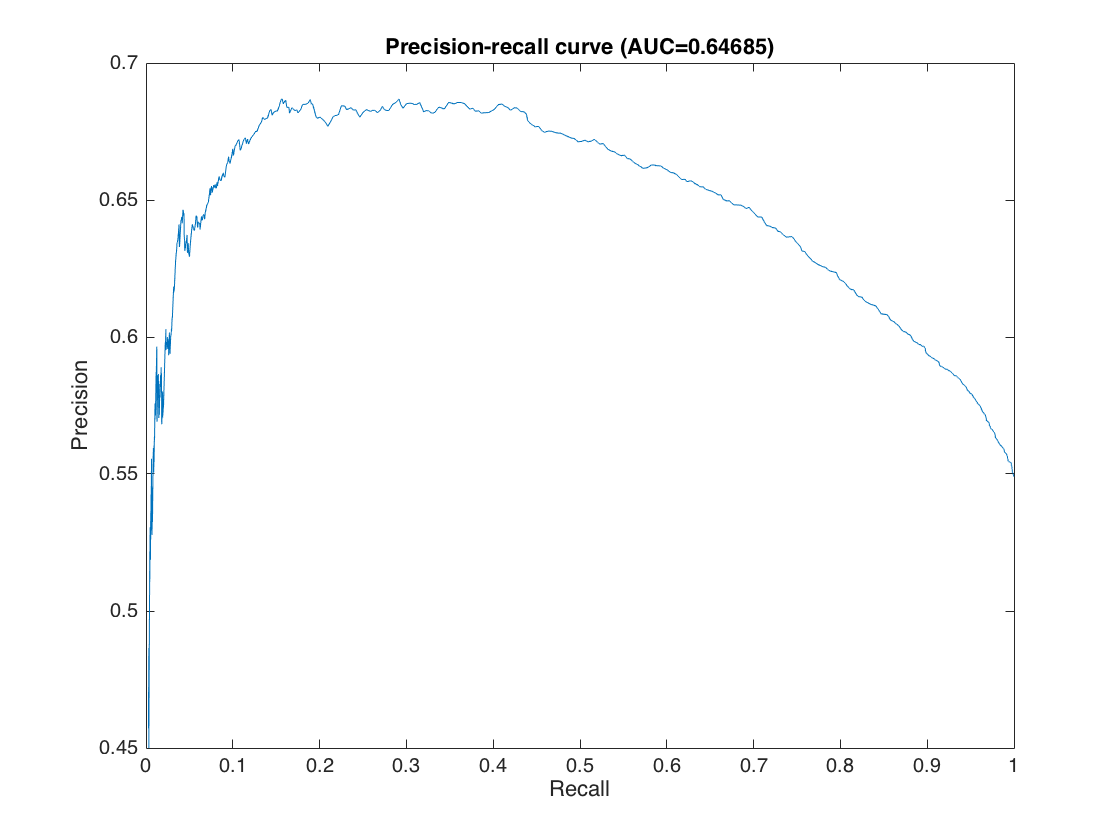
\includegraphics[width=.6\textwidth]{problem3.png}
\caption{Precision verus Recall}
\label{fig:problem3}
\end{figure}
\end{document}